\documentclass{article}
\title{C (PROGRAMMING LANGUAGE)}
\author{OGBODO UDONNA}
\usepackage{graphicx}
\usepackage{graphics}
\begin{document}
	\section{HISTORY and THE FOUNDER } C programming language was developed in the year 1972 at Bell Labs by Dennis Ritchie an American computer scientist. 
\begin{figure}
	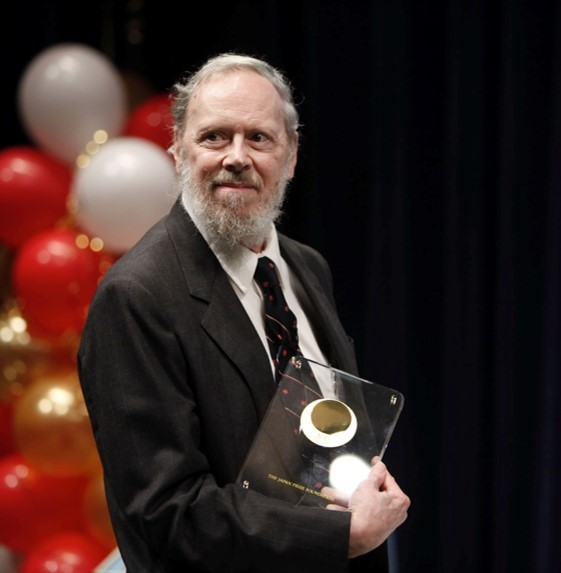
\includegraphics{DENNISM}
	\caption{ \underline{DENNIS RITCHIE}}
	\label{fig:dennism}
\end{figure}
\section{HISTORY OF C} The interesting thing about the history of the C programming language is how it came about. The programming language was created as a means of system implementation for the UNIX operating system.
So before the C programming language came into play Dennis Ritchie and his colleague Ken Thompson wanted to develop a programming language to make utilities for the new UNIX platform so they modified the BCPL system language and then came the development of B programming language.

	
\end{document}